\documentclass[landscape,a0b]{a0poster_csml_v2}
% NOTE: to remove logo from title, just use \headerNoLogo option below
% Options (don't put spaces between options!)
% portrait and landscape: format of the page 
% A0, A1, A2, A3, A4 : size of the poster

% compared to the old mpi poster style, two things have changed: 
% - it now can be compiled with both (ps)latex and pdflatex
% - there are different variants for headers: one with the mpi logos, 
%   and one where you can include arbitrary files as logos (or have no
%   logos at all). 
% 


% if you want to use pdflatex, then include the commands:
\usepackage[pdftex]{graphicx,color}
\DeclareGraphicsExtensions{.pdf}
% if you want to use (ps)latex, then include the commands: 
%\usepackage{graphics}
%\DeclareGraphicsExtensions{.eps}


\usepackage{amssymb,amsmath}
\usepackage{multirow}
\usepackage{booktabs} 

% size of the columns of the poster, relative to the width of the
% whole poster: 
\renewcommand{\columnfrac}{.3}% i.e. want three columns
\newcommand{\half}{\frac{1}{2}}


\definecolor{LimeGreen}{rgb}{0.1,0.9,0.1}
\definecolor{Maroon}{rgb}{0.9,0.1,0.1}

\usepackage{natbib}

\usepackage{listings}

\lstset{language=Matlab,
  basicstyle=\ttfamily\normal,
  keywordstyle=\color{blue}\ttfamily,
  stringstyle=\color{red}\ttfamily,
  commentstyle=\color{green}\ttfamily,
  aboveskip=10pt,
  belowskip=10pt,
  breaklines=true
}



\begin{document}
\begin{poster}

%------------------------------------------------------------
% header: 
%------------------------------------------------------------

% Additionally to the 'normal' font size commands as
% \tiny,\small,\large\ (look them up in a latex book) there are now
% the fonts \veryHuge, \VeryHuge, \VERYHuge

%title: 
\savebox{\PosterTitle}{\VeryHuge Learning to Discover Efficient Mathematical Identities}
%authors:
\savebox{\PosterAuthor}{\Large 
Wojciech Zaremba$^{1, 3}$, Karol Kurach$^{2, 3}$, Rob Fergus$^{1, 4}$}
%addresses:
\savebox{\PosterAddress}{\large 
$^1$Courant Institute NYU; $^2$University of Warsaw; $^3$Google; $^4$Facebook}



% Logos: 

% you can either use the standard MPI header 
% (make sure the logo files logo_mpi.pdf and logo_kyb.pdf are in your
% latex path):
% \headerMpi 

% or you can use a header without any logos: 
\headerNoLogo 

% or you can enter your own logos and use them in the header:
% (make sure the figures are in the path):
%\newcommand{\LeftLogoFile}{example_logo.pdf}
%\newcommand{\RightLogoFile}{example_logo.pdf}
%\headerCustomLogo



% the new color can then be used with the command \color{name}
%\definecolor{anewcolor}{rgb}{0.5,0,0}
%\newcommand{\ulescolor}{\bf \color{anewcolor}}
\definecolor{mpigreen}{rgb}{0.3,0.61,0.59}
\definecolor{mpigrey}{rgb}{0.86,0.85,0.83}
\definecolor{red}{rgb}{1,0,0}
\definecolor{brightgreen}{rgb}{0,1,0}
\definecolor{palepink}{rgb}{1.0,0.4,0.4}
\definecolor{anublue}{rgb}{0,0.5,0.9}
\definecolor{blue}{rgb}{0,0,1}
\definecolor{engPink}{cmyk}{0.0,0.4,0.44,0.33}


\newcommand{\Mpigreen}[1]{\color{mpigreen}{#1}\color{black}}
\newcommand{\Mpigrey}[1]{\color{mpigrey}{#1}\color{black}}
\newcommand{\Red}[1]{\color{red}{#1}\color{black}}
\newcommand{\Brightgreen}[1]{\color{brightgreen}{#1}\color{black}}
\newcommand{\Palepink}[1]{\color{palepink}{#1}\color{black}}
\newcommand{\Anublue}[1]{\color{anublue}{#1}\color{black}}
\newcommand{\Blue}[1]{\color{blue}{#1}\color{black}}
\newcommand{\Engpink}[1]{\color{engPink}{#1}\color{black}}



%Maths macros
\newcommand{\bdatax}{\mathbf{X}}
\newcommand{\bdatay}{\mathbf{Y}}
\newcommand{\bdata}{\mathbf{Z}}

\newcommand{\Eb}{\mathbf{E}}
\newcommand{\Ex}{\mathbf{E}}
\renewcommand{\Pr}{\boldsymbol{\mathsf{P}}}
\newcommand{\Qr}{\boldsymbol{\mathsf{Q}}}

\newcommand{\Fcal}{\mathcal{F}}
\newcommand{\Xcal}{\mathcal{X}}
\newcommand{\Ycal}{\mathcal{Y}}

%DEBUG: re-introduce when compiling on laptop
%\renewcommand{\Re}{\mathbb{R}}
\newcommand{\Nat}{\mathbb{N}}

\newcommand{\sx}{\mathsf{x}}
\newcommand{\sy}{\mathsf{y}}
\newcommand{\sz}{\mathsf{z}}

\newcommand{\BigO}[1]{\ensuremath{\operatorname{O}\left(#1\right)}}

% ------------------------------------------------------------
% first column: 
% ------------------------------------------------------------
% Attention: between the end of one column and the begin of the next
% column must not be spaces - otherwise latex thinks that it has to
% make a pagebreak... see below how I did it!


\begin{PosterColumn} 
  
\PosterBox{The Combinatorial Explosion \\ Discrete search is a central issue in AI}

\vspace{-2cm}
\begin{center}
\end{center}
\vspace{0.5cm}
\begin{minipage}[hc]{0.19\textwidth}
  \centering
  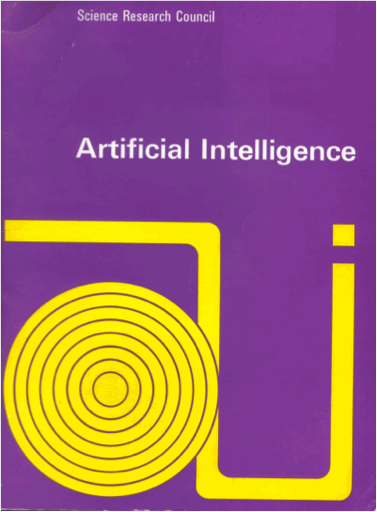
\includegraphics[width=0.95\linewidth]{imgs/book.png}
  \\
\end{minipage}
\hfill
\begin{minipage}[hc]{0.8\textwidth}
  From ``Artificial Intelligence: A General Survey'' by Professor Sir James Lighthill, 1973. \\
  \vspace{0.5cm}
  \\
  ``...failure to recognize the implications of the {\bf \textcolor{red}{combinatorial~explosion}}. This is a general obstacle to the construction of a self-organising system on a large knowledge base which results from the explosive growth of any combinatorial expression, representing numbers of possible ways of grouping elements of the knowledge base according to particular rules, as the base's size increases.''
\end{minipage}

\vspace{0.7cm}

\PosterBox{Math \& Theorem Proving}

\begin{minipage}[hc]{0.45\textwidth}
  {\bf Contemporary theorem provers}
  \begin{itemize}
    \item Requires search over all possible combinations of operators
    \item Intractable for all but simple proofs
    \item Automated Theorem Provers use heuristics
  \end{itemize}
\end{minipage}
\hfill
\begin{minipage}[hc]{0.45\textwidth}
  {\bf Yet (some) humans are able to prove theorems}
  \vspace{0.5cm}
  \begin{itemize} 
    \item Have experience of related problems 
    \item Known math ``tricks''
  \end{itemize} 
\end{minipage}

\vspace{1.2cm}
We focus on simpler problem: discovering identities in mathematics.

\PosterBox{Toy Example}

\begin{minipage}[hc]{0.45\textwidth}
  \centering
  Consider two matrices $A$ and $B$:
  \begin{align*}
    \sum_{i, k}(AB)_{i, k} = \sum_i \sum_j \sum_k a_{i,j} b_{j, k}
  \end{align*}
\end{minipage}
\hfill
\begin{minipage}[hc]{0.45\textwidth}
  \centering
  Naive computation takes $\BigO{n^3}$: 
  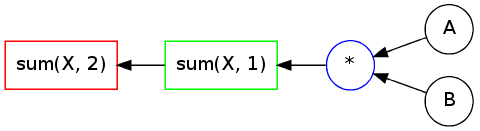
\includegraphics[width=0.9\linewidth]{imgs/example1_brute.png}
\end{minipage}
\vspace{1cm}

\PosterBox{Discovering Efficient Identities}
Define a grammar G of operators
Given some target expression $T$ within the domain of $G$
e.g. sum(sum(A*B,2),1). Find an identical expression that has lower computational 
complexity i.e. avoids high complexity operators (like matrix multiplication).
\vspace{1cm}

\begin{minipage}[hc]{0.47\textwidth}
  \begin{center}
    \begin{tabular}{ll}
      \hline
      Matrix-matrix multiply   \hspace{1cm}   &  X * Y \\
      Matrix-vector multiply      & X * y \\
      Matrix-element multiply     & X .* Y \\
      Matrix transpose            & X’ \\
      Column-sum                  & sum(X,1) \\
      Row-sum                     & sum(X,2) \\
      Column-repeat               & repmat(X,1,m) \\
      Row-repeat                  & repmat(X,n,1) \\
      \hline
    \end{tabular}
  \end{center}
\end{minipage}
\hfill
\begin{minipage}[hc]{0.47\textwidth}
\begin{center}
Polynomials of degree 1
\end{center}
\begin{align*}
  A, A^T, \sum_i A_{i, :}, \sum_j A_{:, j}, \sum_{i, j} A_{i, j}, \dots 
\end{align*}
\begin{center}
Polynomials of degree 2
\end{center}
\begin{align*}
  A^2, (A^2)^T, AA^T, A^TA, \sum_i (AA^T)_{i, :}, \dots \\
\end{align*}
\end{minipage}
\vspace{-1cm}
\begin{center}
  {\bf Space grows exponentially fast.}
\end{center}
\vspace{-1cm}

\PosterBox{Representing Symbolic Expressions}
Target expression: sum(sum(A*A’,1),2)
Use $P$ copies of $A$


Representation of target is descriptor vector (length $P$)
\begin{itemize}
  \item Each element is evaluation one copy
  \item Vector is of length $P$
  \item If descriptors match equivalent expressions.
\end{itemize}

Using is unstable, so use      
integers modulo $q$, where $q$ is large prime.




\end{PosterColumn}
\begin{PosterColumn} 

\PosterBox{Example: Taylor Series Approximation}

\begin{minipage}[hc]{0.57\textwidth}
  Consider RBM partition function:
  \begin{align*}
    \sum_{v,h} \exp(v^TWh) = \sum_{k=0}^\infty \sum_{v,h} \frac{(v^TWh)^k}{k!}\\
    v \in \{0, 1\}^n\\
    h \in \{0, 1\}^m
  \end{align*}
  {\bf 1st term in Taylor series:}
  \begin{align*}
    \sum_{k=0}^\infty \sum_{v,h} v^TWh = 2^{n + m - 2} \sum_{i, j}W_{i, j}
  \end{align*}
\end{minipage}
\hfill
\begin{minipage}[hc]{0.37\textwidth}
  \centering
  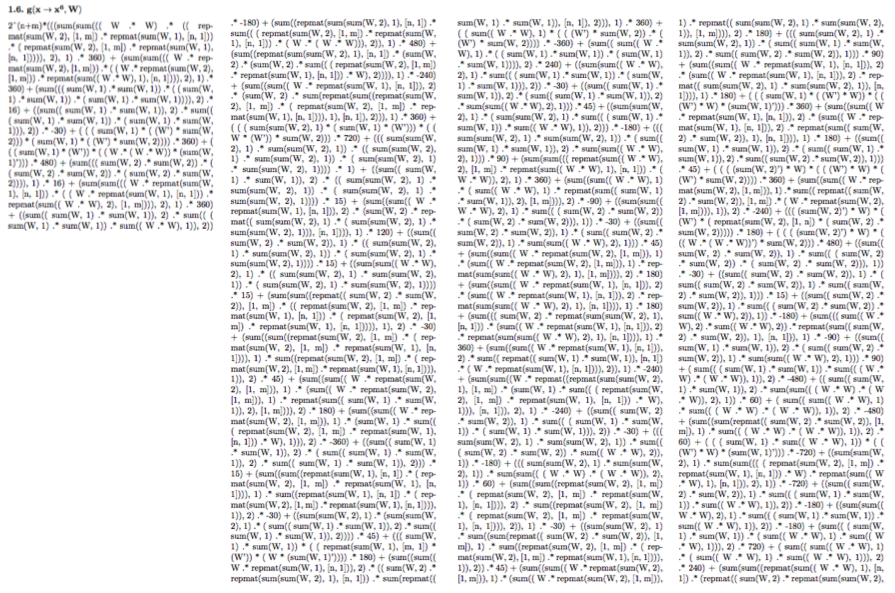
\includegraphics[width=\linewidth]{imgs/6th.png}
  6th term.
  Higher terms too complex for manual derivation. 
\end{minipage}
\vspace{0.5cm}
\\

  {\bf 2st term in Taylor series:}
  \begin{align*}
    \sum_{k=0}^\infty \sum_{v,h} (v^TWh)^2 = 2^{n + m - 4} [\sum_{i, j}W_{i, j}^2 + (\sum_{i, j} W_{i, j})^2 + \sum_i (\sum_j W_{i, j})^2 + \sum_j (\sum_i W_{i, j})^2]
  \end{align*}
  Note that identity computes in $\BigO{nm}$ versus $\BigO{2^{n + m}}$ for original expression.
\vspace{0.7cm}


\PosterBox{Prior Over Computation Trees}

Recall goal: find equivalent expressions to target
i.e. descriptors match
Restrict grammar to use operators with lower complexity than target
If any match found then sure to be efficient w.r.t. target
\vspace{-0.8cm}
\begin{center}
{\bf Want to learn a good \textcolor{red}{prior} over expressions}
\end{center}

\vspace{-0.2cm}
\textcolor{anublue}{Scheduler} picks potential new operators to append to current expression(s).

Example:

\begin{minipage}[hc]{0.45\textwidth}
  \centering
  Current expression: \\
  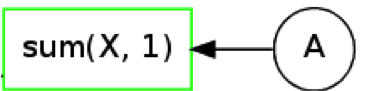
\includegraphics[width=0.5\linewidth]{imgs/current.png}
\end{minipage}
\hfill
\begin{minipage}[hc]{0.45\textwidth}
  \centering
  Valid operators to append:\\
  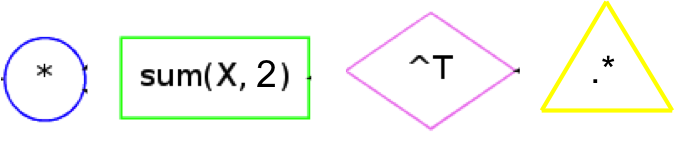
\includegraphics[width=0.8\linewidth]{imgs/possible.png}
\end{minipage}
\vspace{1.5cm}
\\
\textcolor{mpigreen}{Scorer} ranks each possibility (i.e. how likely they are to lead to the solution), using {\bf \textcolor{red}{prior}}.
\vspace{0.5cm}
\\
\begin{minipage}[hc]{\textwidth}
  \begin{center}
    \begin{tabular}{lll}
      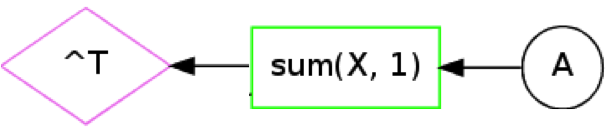
\includegraphics[width=0.2\linewidth]{imgs/prior1.png} \hspace{4cm} & Score 0.3 \\
                                                                          & & \\
      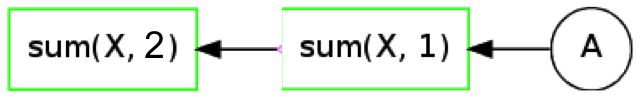
\includegraphics[width=0.2\linewidth]{imgs/prior2.png}  & Score 0.05 \\
                                                                          & & \\
      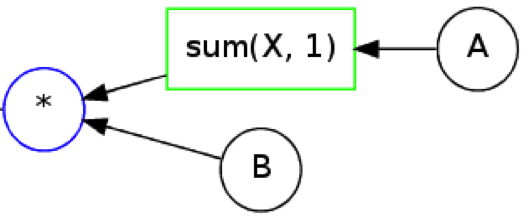
\includegraphics[width=0.2\linewidth]{imgs/prior3.png}  & Score 0.65 \\
    \end{tabular}
  \end{center}
\end{minipage}
\vspace{0.5cm}
\\
Sample new operator according to scorer probabilities

\PosterBox{Scorer Strategy}
\vspace{-1cm}
\begin{itemize}
  \item Naive: no prior, Just select randomly from all valid operators
  \item $n$-gram prior
  \item Recurrent Neural Network prior
\end{itemize}

Use curriculum learning approach.
Start with easy targets, and uniform prior (low polynomial degree $k$). 
Refine prior using new solution.
\vspace{0.5cm}
\\
\begin{minipage}[hc]{\textwidth}
  \begin{center}
    \begin{tabular}{lll}
      \hline
        & Target Expression & Efficient expression \\
      \hline
      K = 1 \hspace{1cm} & $\sum_i a_i \hspace{1cm} $ & sum(sum(A, 1), 2) \\
      \hline
      K = 2 & $\sum_{i,j} a_ia_j $ & 0.5 * (sum((repmat(sum(A', 1), 1, m) .* A), 2)) + \\
            & & -0.5 * (sum((A .* A)', 1))) \\
      \hline
      K = 3 & $\sum_{i, j, k}a_ia_ja_k$ & (-0.5 * (sum((repmat(sum((A' .* A'), 1), 1, m) .* A), 2)) + \\
      & & 1/3 * (sum(((A' .* A')' .* A), 2)) + \\
      & & 1/6 * (sum((A' .* repmat(sum((repmat( \\
      & & sum(A', 1), 1, m) .* A), 2), m, 1)), 1))) \\
      \hline
    \end{tabular}
  \end{center}
\end{minipage}

\end{PosterColumn}
\begin{PosterColumn} 

\PosterBox{$n$-gram}
\begin{minipage}[hc]{\textwidth}
  \centering
  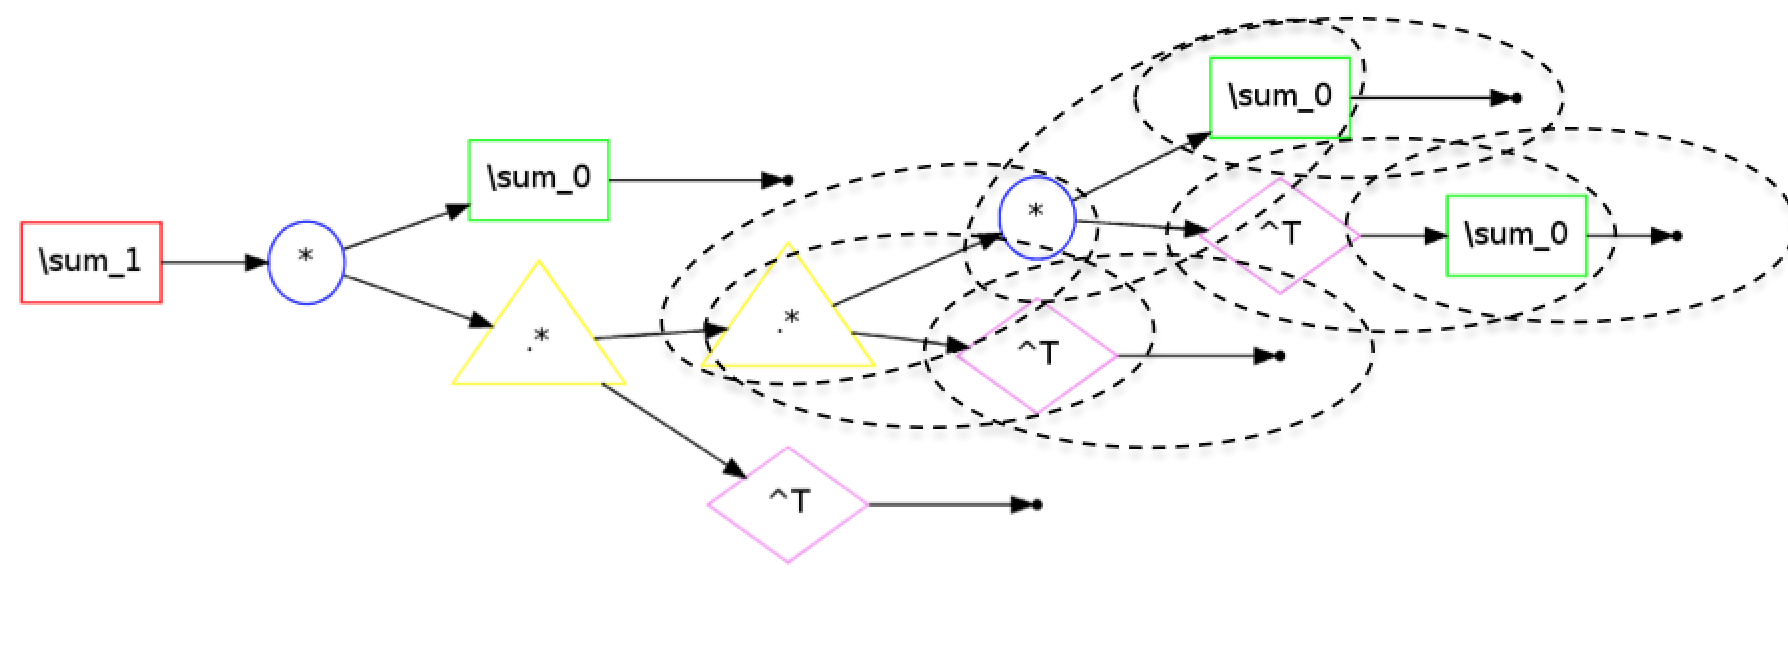
\includegraphics[width=0.40\linewidth]{imgs/bigram.png}
  \hfill
  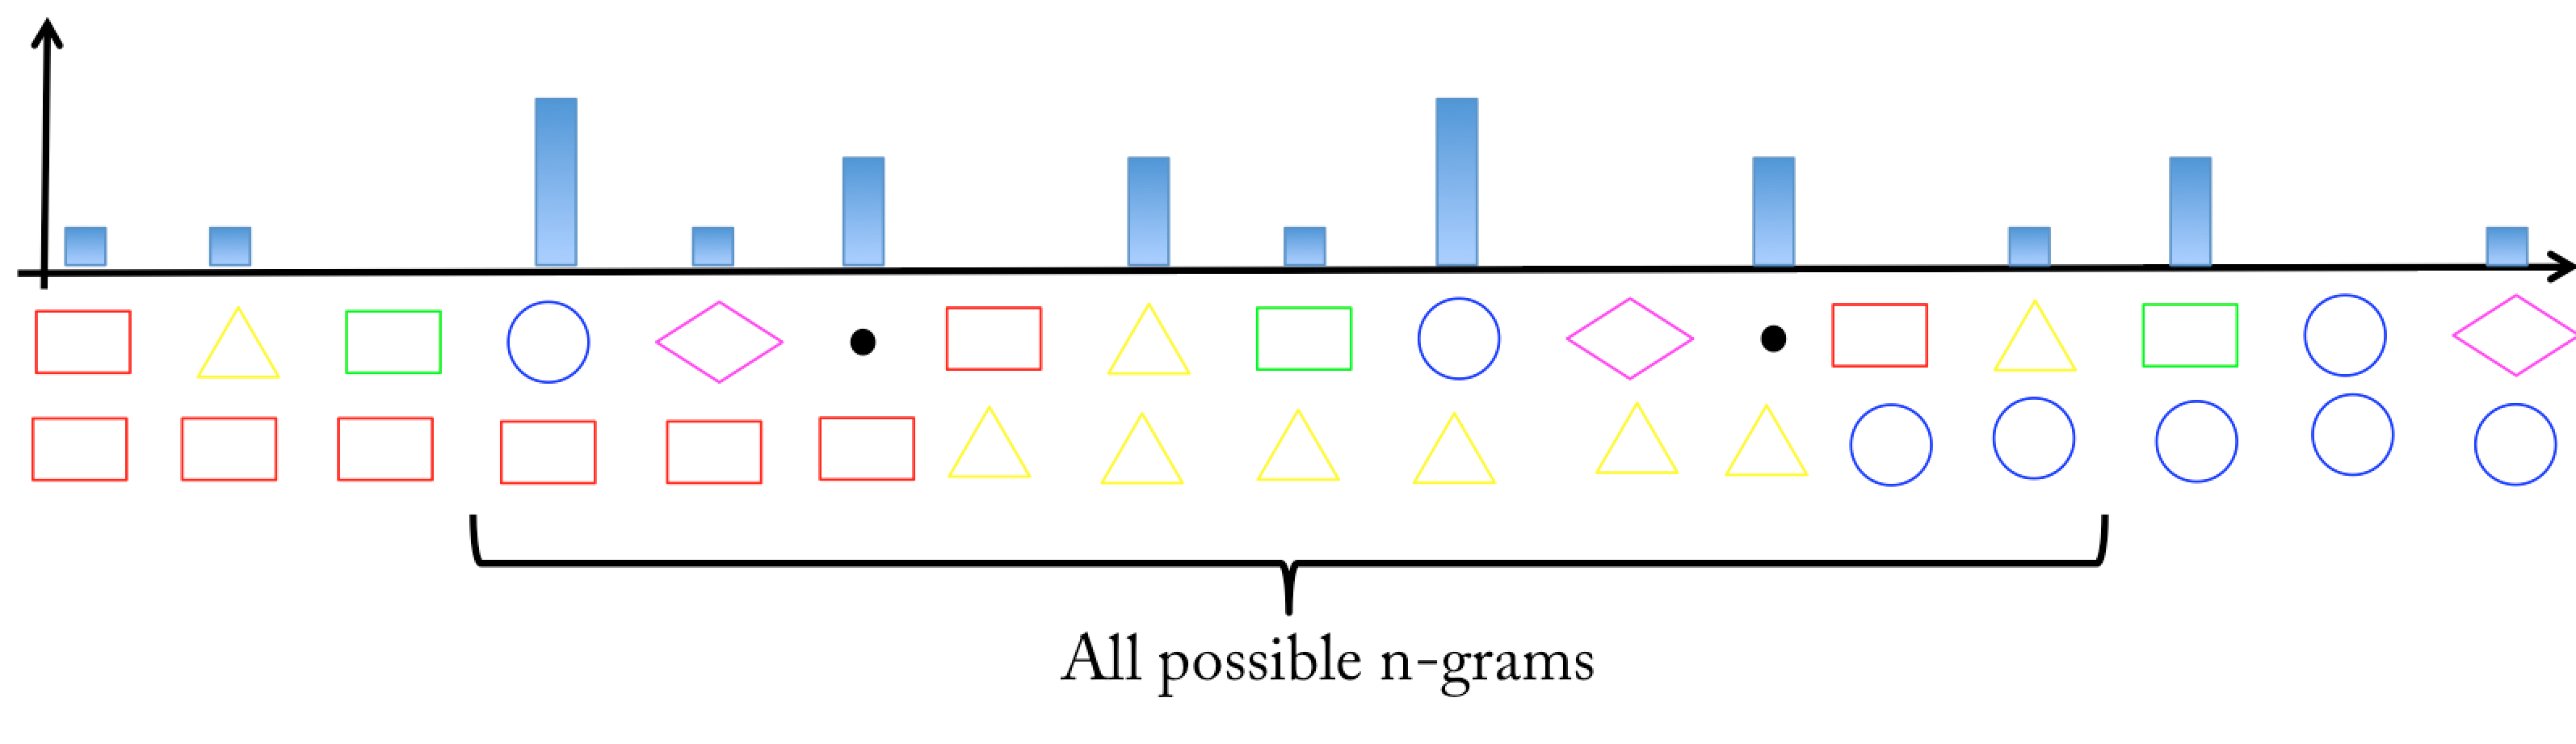
\includegraphics[width=0.40\linewidth]{imgs/histogram.png}
\end{minipage}

\PosterBox{Experiments in discovering identities}
$5$ families of expressions (vary degree $k$)
\begin{itemize}
  \item Multiply-sum: $\sum (AA^T)_k$
  \item Element-wise multiply-sum: $\sum ((A.* A)A^T)_k$
  \item Symmetric polynomials: $\sum_{i, j, k} a_ia_ja_k$
  \item RBM-1: $\sum_{v \in \{0, 1\}^n} (v^tA)^k$
  \item RBM-2: $\sum_{v \in \{0, 1\}^n, h \in \{0, 1\}^m} (v^tAh)^k$
\end{itemize}


Start with $k=1$ and work up to $k=15$.
Time cut-off: $600$ seconds
Repeat $10$ times, measure fraction successful


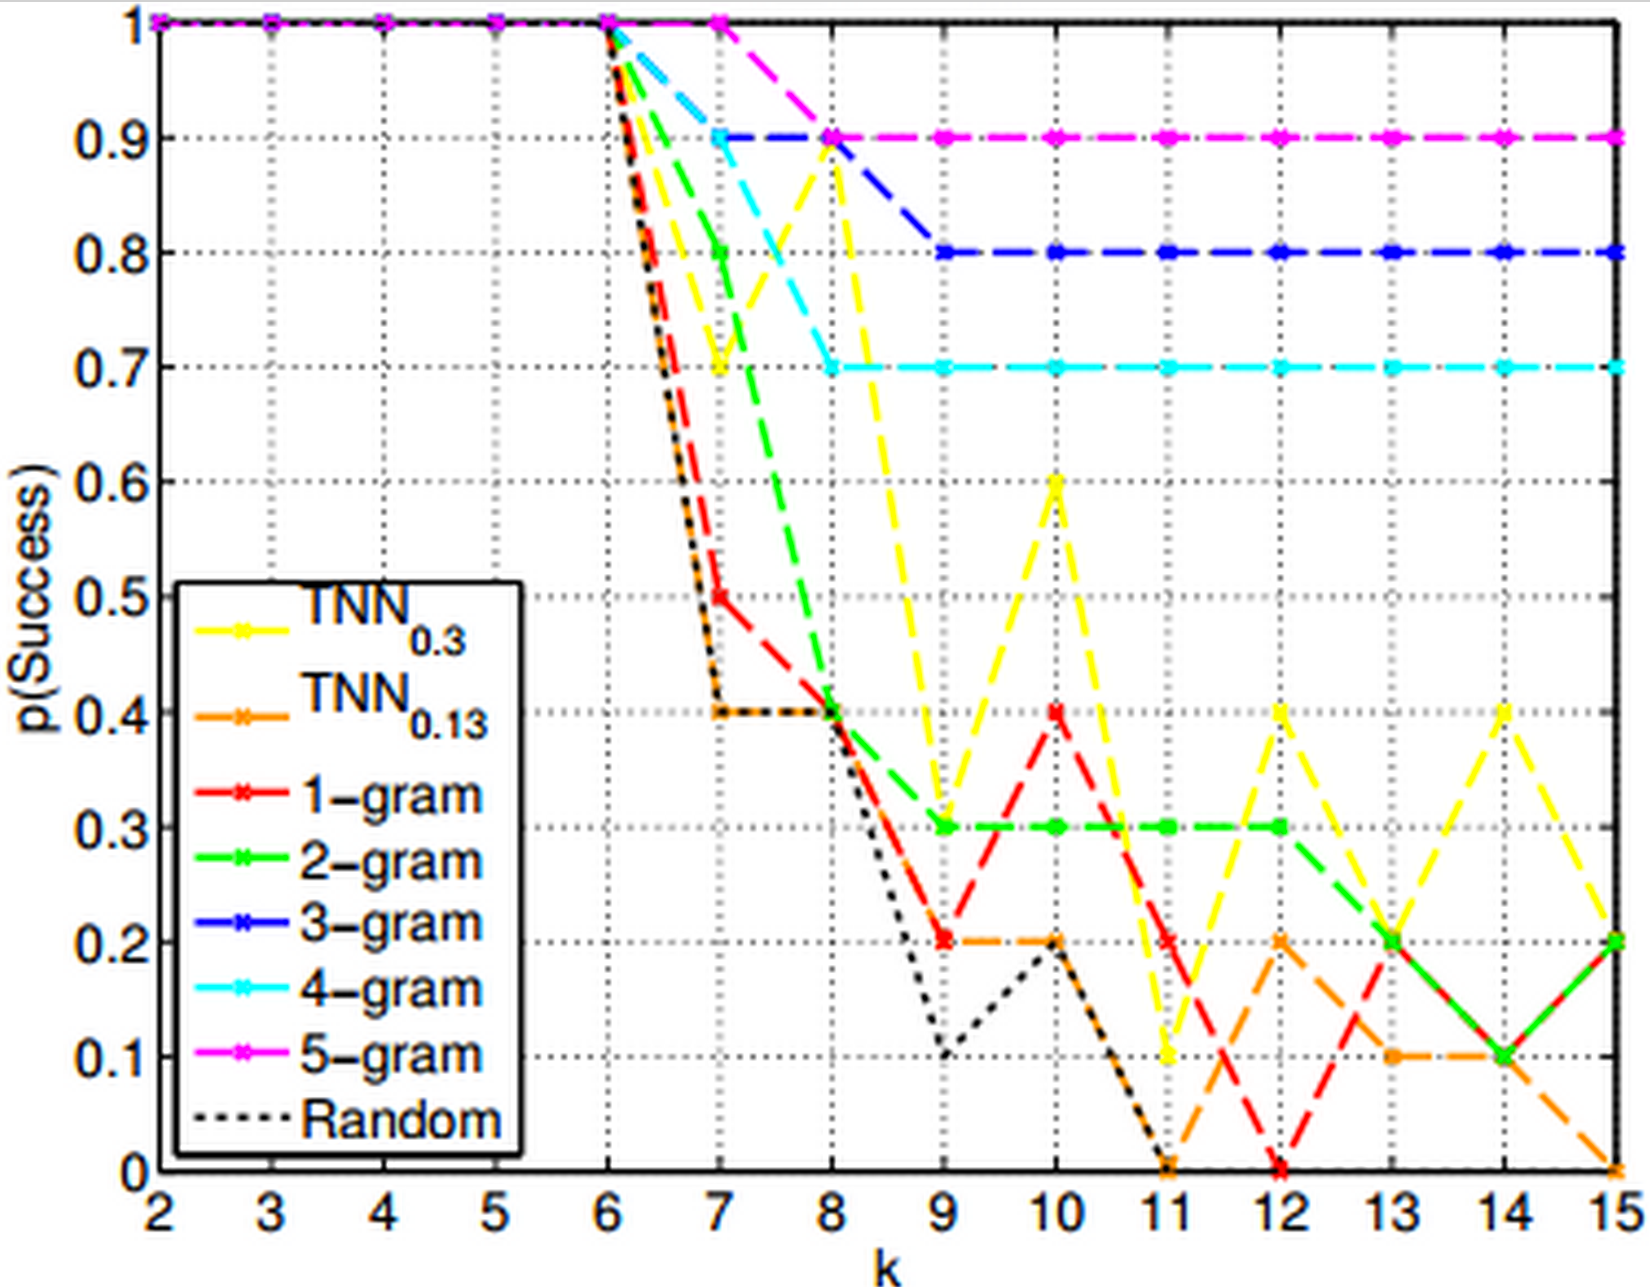
\includegraphics[width=0.24\linewidth]{imgs/plot_aat.png}
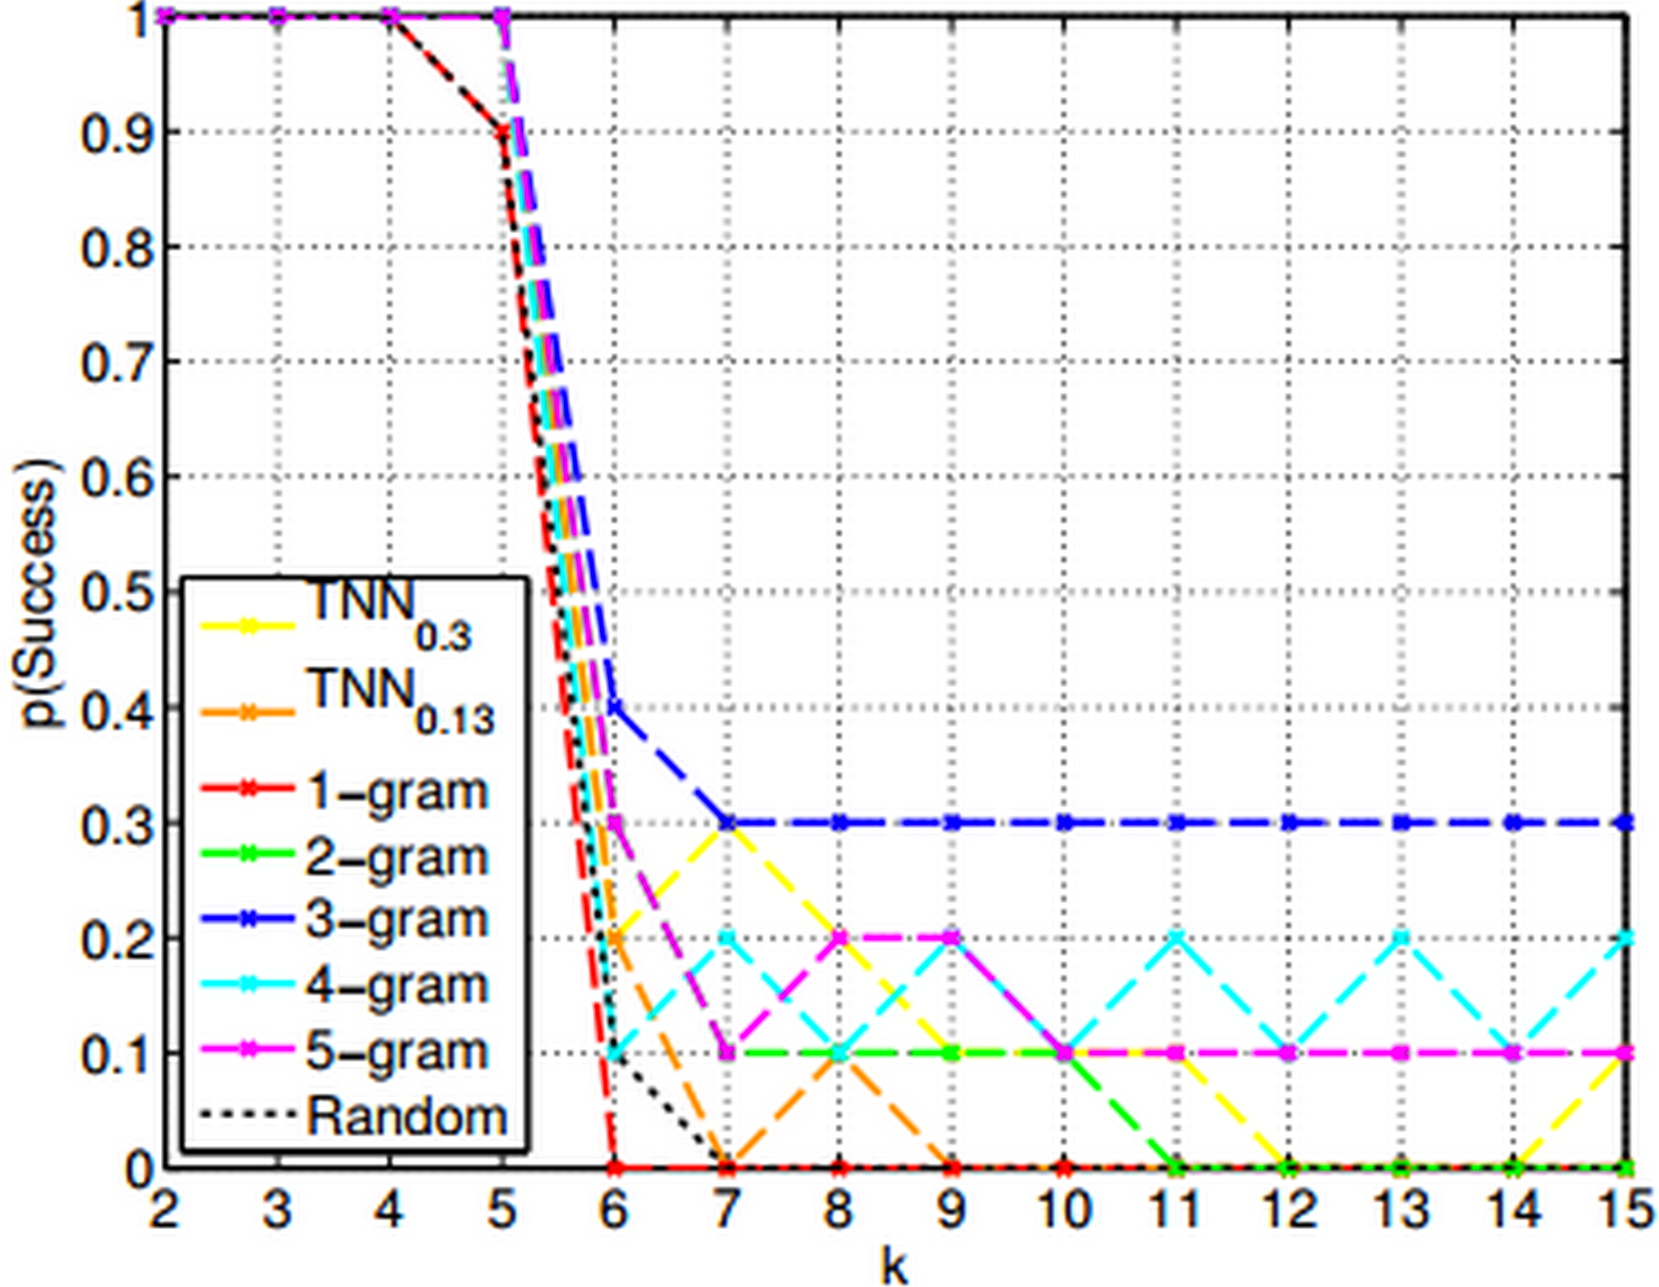
\includegraphics[width=0.24\linewidth]{imgs/plot_aaa.png}
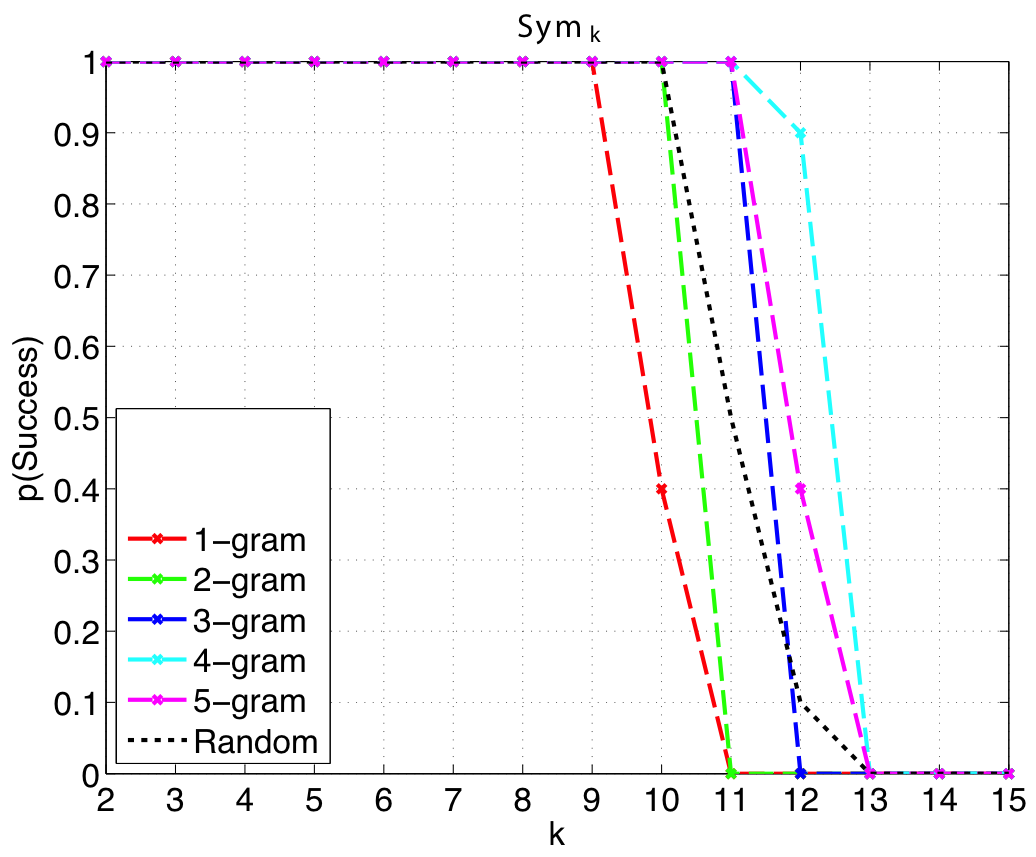
\includegraphics[width=0.24\linewidth]{imgs/plot_sym.png}
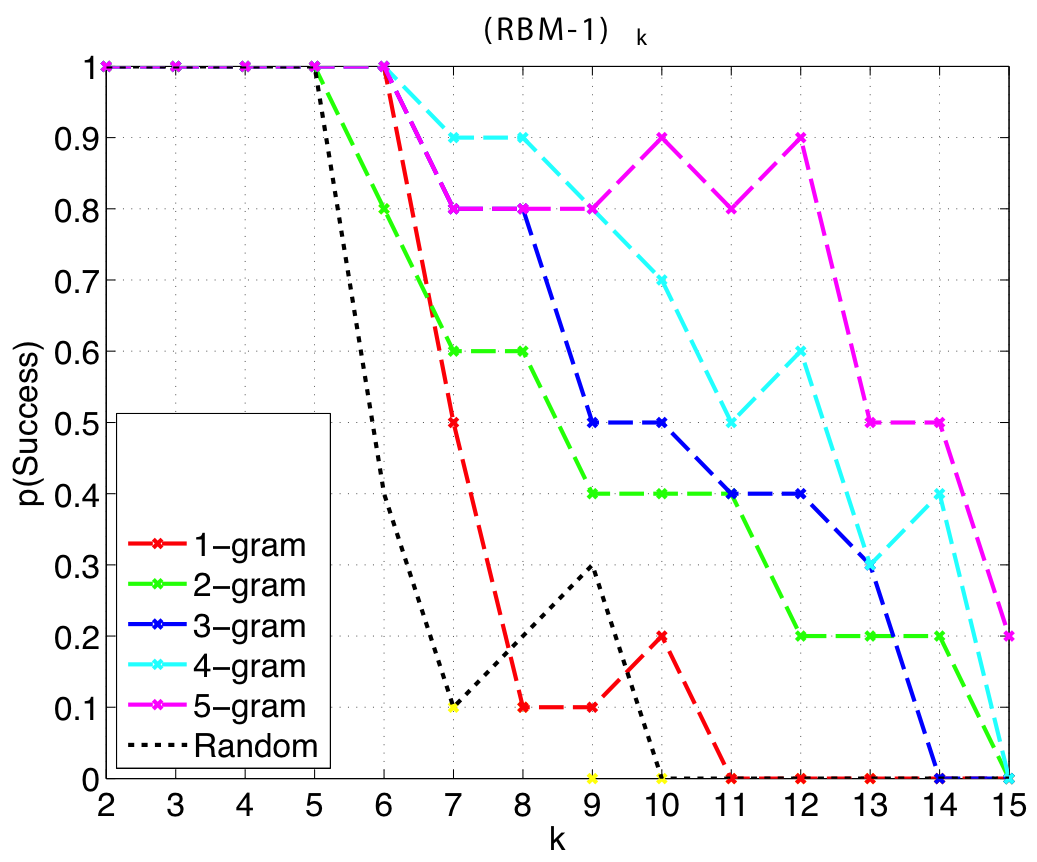
\includegraphics[width=0.24\linewidth]{imgs/plot_rbm1.png}
\\
{\bf RBM-2}\\
No scorer strategy able to get beyond $k=5$ 
However, the $k = 5$ solution was found by the RNN consistently faster than the random strategy ($100 \pm 12$ vs $438 \pm 77$ secs). 
\PosterBox{Recurrsive neural network strategy}
$n$-gram has a shallow understanding of mathematical expressions (up to depth $n$).
We trained recurrsive neural network to identify equivalent expressions.
\begin{minipage}[hc]{\textwidth}
  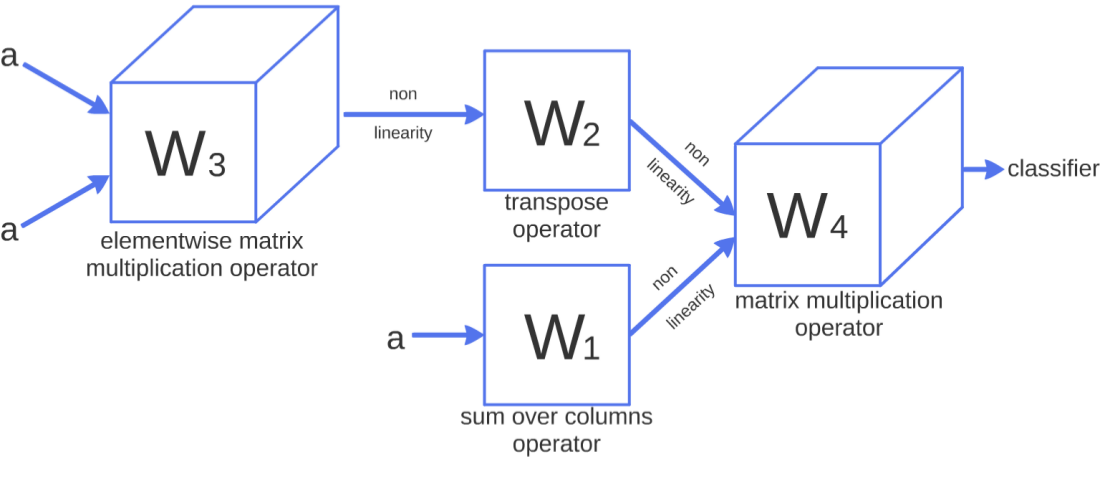
\includegraphics[width=0.45\linewidth]{imgs/tnn.png}
  \hfill
  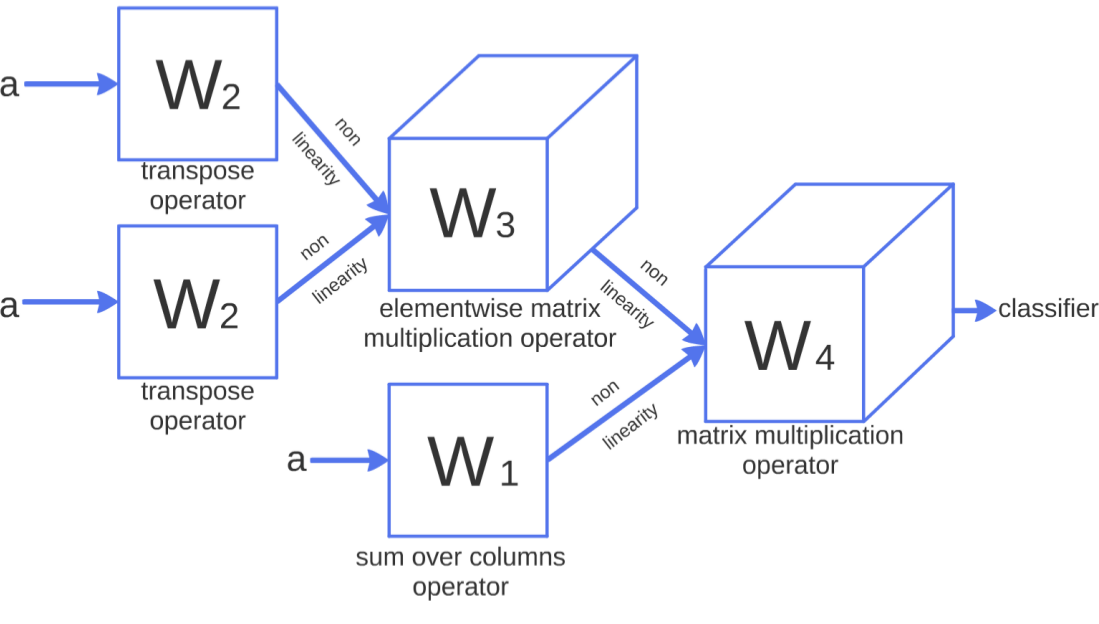
\includegraphics[width=0.45\linewidth]{imgs/tnn2.png}
\end{minipage}

\begin{itemize}
  \item Training data: for each degree find groups of equivalent expressions (exhaustive search).
  \item Label each group as a different class.
  \item Add softmax classifier to RNN and train with cross-entropy loss.
\end{itemize}

Training examples for degree k=6:\\
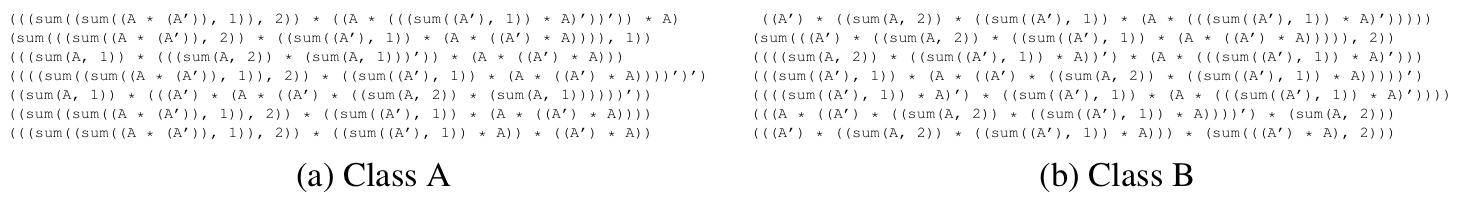
\includegraphics[width=0.98\linewidth]{imgs/classes.png}
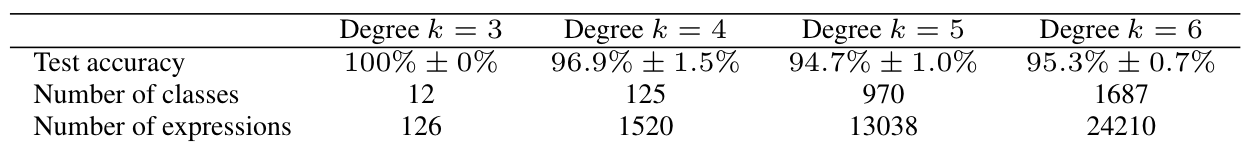
\includegraphics[width=0.98\linewidth]{imgs/print_trees.png}
\vspace{-0.5cm}
\begin{center}
Note: no explicit knowledge of math operators
\end{center}
\vspace{-0.5cm}
\PosterBox{Related work}
\vspace{-0.8cm}
\begin{itemize}
  \item Recent efforts to combine ML with theorem provers, e.g. Bridge et al. 2014
  \item Distilling Free-Form Natural Laws from Experimental Data, Michael Schmidt and Hod Lipson.  Science, Vol. 324, April 3, 2009.
  \item Recursive neural nets in NLP Socher et al. 2013, Luong et al., learning logics Bowman et al. 2014 for logical predicates
  \item Learning to Execute, Wojciech Zaremba \& Ilya Sutskever, arXiv 1410.4615, 2014
\end{itemize}
\end{PosterColumn}

%%%
\end{poster}
\end{document}



